\documentclass[../report.tex]{subfiles}
\begin{document}	
	
\chapter{Optical waveguide theory}
To understand the working principle of \gls{pr} it is important to look into the basic concepts of waveguides and the mathematics behind the propagation of \gls{em} waves. Maxwell combined the electric and magnetic fields in a wave equation for a homogeneous medium. Moreover, to understand \gls{pr} in waveguides, it also necessary to look into polarization of light and its formal representation using Jones Calculus. Additionally, Poincaré sphere and Stoke's parameter are required for a representation of \gls{sop}. Apart form these, different \gls{fom} parameters are used to describe transmission parameters in a waveguide.   
		
	\section{Maxwell's equations}
A wave is a disturbance that propagates through a medium. Waves transfer both energy and momentum, without transferring any mass. \gls{em} radiation is the radiant energy released by varying \gls{em} field in the form of \gls{em} waves. A light wave is \gls{em} radiation at very high frequency. The frequency of visible light falls in between IR and UV \gls{em} waves.
\begin{figure}[h]
	\centering
	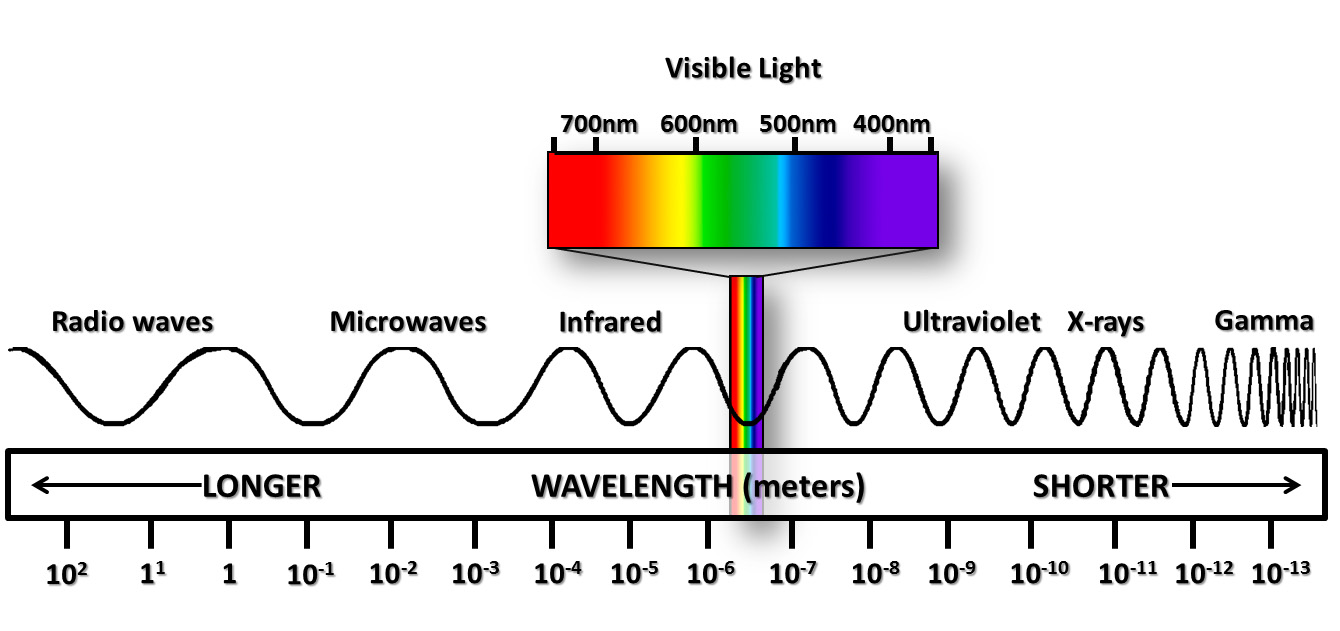
\includegraphics[width=0.75\textwidth]{2-light-spectrum}
	\caption{The \gls{em} wave spectrum}
	\label{fig:2_light_spectrum}
\end{figure}
James Clerk Maxwell discovered that he could combine four simple equations, which had been previously discovered, along with a slight modification to describe self-propagating waves of oscillating electric and magnetic fields \cite{waveparticle_2016}. The understanding of propagating light waves using Maxwell's equations in a dielectric medium, is the key to the construction of waveguides. Maxwell’s equations relate the electric field $E$ (V/m), magnetic field $H$ (A/m), charge density $\rho$ ($\chem{C/m^3}$), and current density $J$ ($\chem{A/cm^2}$).
\begin{itemize}	
	\item \textbf{Maxwell's first equation (Gauss' Law)}: The net electric flux through any closed surface is equal to $\frac{1}{\epsilon_m}$ times the charge density within that closed surface,
	\begin{equation}\label{eq:max1_1}
	\nabla \cdot \vec{E} = \frac{\rho}{\epsilon_m},	
	\end{equation}
	where $\epsilon_m$ the permittivity of the medium, and the del operator, $\nabla$, is given by:
	\begin{equation}\label{eq:max1_2}
	\nabla = \left(\frac{\partial i}{\partial x},\frac{\partial j}{\partial y},\frac{\partial k}{\partial z}\right)
	\end{equation}
	where i, j and k are unit vectors in the x, y and z directions respectively.
	
	\item \textbf{Maxwell's second equation (Gauss' Law for magnetic field)}: The net magnetic flux through a closed surface is always zero, since magnetic monopoles do not exist.
	\begin{equation}\label{eq:max1_3}
	\nabla \cdot \vec{H}= 0	
	\end{equation}
	
	\item \textbf{Maxwell's third equation (Faraday's law)}: Induced electric field around a closed path is equal to the negative of the time rate of change of magnetic flux enclosed by the path.
	\begin{equation}\label{eq:max1_4}
	\nabla\times \vec{E} = -\mu_m\frac{\partial \vec{H}}{\partial t}
	\end{equation}
	where $\mu_m$ is the magnetic permeability of the medium.

	\item \textbf{Maxwell's fourth equation (Modification of Ampere's law)}:  The fourth equation states that magnetic fields can be generated in two ways: by electric current (this was the original “Ampere's law”) and by changing electric fields (this was “Maxwell's addition”) \cite{wiki_maxwells_2016}.
	\begin{equation}\label{eq:max1_5}
	\nabla\times \vec{H} =  J + \epsilon_m\frac{\partial \vec{E}}{\partial t}	
	\end{equation}
	where $\epsilon_m$ is the electric permittivity of the medium.	
\end{itemize}

\noindent These equations combine into the following wave equation
\begin{equation}\label{eq:wave_eq}
\nabla^2 \vec{E} -  \mu_m\epsilon_m\frac{\partial^2 \vec{E}}{\partial t^2} = \mu_m\frac{\partial J}{\partial t} + \frac{\nabla\rho}{\epsilon_m},	
\end{equation}
using the curl of curl identity operation given by, 
\begin{equation}\label{eq:curl_of_curl}
\nabla^2 \vec{E} = \nabla(\nabla \cdot \vec{E}) - \nabla\times(\nabla\times \vec{E}).
\end{equation}
A general solution to the equation \ref{eq:wave_eq} in free space, in absence of charge is,
\begin{equation}\label{eq:wave_sol_electric}
\vec{E}(z,t)=E_{0}(x,y)e^{i\left(\omega t \pm k_{0}z\right)},
\end{equation}
where $z$ is direction of propagation of wave in Cartesian coordinates, phase $\phi$ = $\omega t \pm k_{0}z$ and wave vector propagation constant, $k_0$ = $\dfrac {\partial \phi } {\partial t}$ = $\dfrac {2\pi } {\lambda }$, in the direction of propagation of the wave. Similar calculations for the magnetic field, $\vec{H}$ in free space yields, 		
\begin{equation}\label{eq:wave_sol_magnetic}
\vec{H}(z,t)=H_{0}(x,y)e^{i\left(\omega t \pm k_{0}z\right)}
\end{equation}

\section{Transverse electromagnetic wave}
\noindent In the Fig. \ref{fig:2_em_wave} the electric field and magnetic field propagate in directions perpendicular to each other. Moreover, the direction of propagation is also transverse to the \gls{em} field. Hence it is called \gls{tem} wave. This is a special case of the wave equation in \ref{eq:wave_eq}.
\begin{figure}[H]
	\centering
	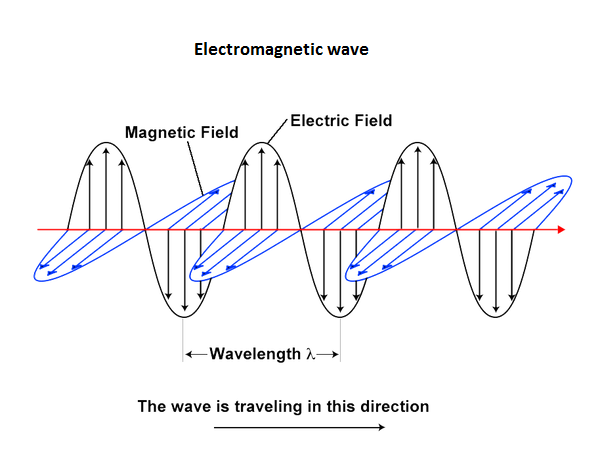
\includegraphics[width=0.75\textwidth]{2-em-wave}
	\caption{Propagation of \gls{tem} wave}
	\label{fig:2_em_wave}
\end{figure}
		\section{Optical waveguides}
The waveguide is the essential element of every photonic circuit, and can be characterized by the number of dimensions in which light is confined inside it \cite{reed_silicon_2008}. A planar waveguide confines light in 1-D, which is simple for understanding of the wave propagation using Maxwell's equations. However, for practical applications 2-D confinement is necessary and that is why channel waveguides are used. Structures like photonic crystals and waveguide cavities even have 3-D confinement properties. The propagation constant in waveguide varies according to $\chem{\textit{n}_{eff}}$, the effective \gls{ri} of the waveguide and is given by 
\begin{equation}\label{eq:propagation_const_med_val}
k = n_{eff}k_0,
\end{equation}
where,
\begin{equation}\label{eq:ri_med_val}
n_{eff} = \sqrt {\varepsilon _{m}\mu _{m}}.
\end{equation}  			
		\subsection{Planar waveguides}
A simple planar waveguide consists of a high-index medium with height $h$ surrounded by lower-index materials on the top and bottom sides, known as cladding. Planar waveguides are also called slab waveguides. The \gls{ri} of the film is $\chem{\textit{n}_{f}}$. The \gls{ri} of the substrate in lower cladding is $\chem{\textit{n}_{s}}$ whereas, \gls{ri} of the substrate in upper cladding is $\chem{\textit{n}_{c}}$.
\begin{figure}[H]
	\centering
	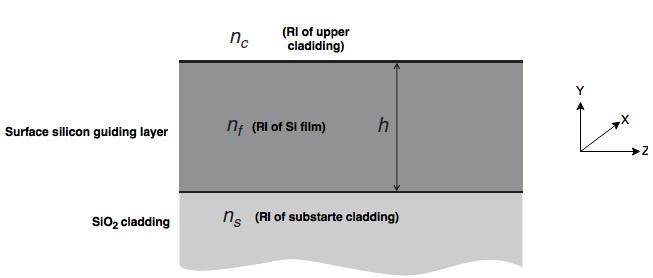
\includegraphics[width=0.75\textwidth]{2-palne-wg}
	\caption{A typical planar waveguide where the film is infinite in XZ-plane}
	\label{fig:2_palne_wg}
\end{figure}
For planar waveguides the wave equation for electric field (\ref{eq:wave_sol_electric}) and magnetic field (\ref{eq:wave_sol_magnetic}) can be rewritten as follows:
\begin{equation}\label{eq:wave_sol_planar_wg}
\begin{aligned}
\begin{cases}
\vec{E}(z,t)=E_{x}(y)e^{i\left(\omega t \pm k_{0}z\right)}\\
\vec{H}(z,t)=H_{x}(y)e^{i\left(\omega t \pm k_{0}z\right)}
\end{cases}
\end{aligned}
\end{equation}	
since in X-direction the film is infinite. After using the homogeneous wave equations for a planar waveguide the following \gls{te} and \gls{tm} mode equations can be deduced:
\begin{equation}\label{eq:homogeneous_wave_sol_planar_wg}
\begin{aligned}
\begin{cases}
\nabla^{2}E_x(y) + (k_{0}^{2}n(y)^{2}-k^{2}){E_{x}(y)} = 0\\
\nabla^{2}H_x(y) + (k_{0}^{2}n(y)^{2}-k^{2}){H_{x}(y)} = 0	
\end{cases}
\end{aligned}
\end{equation}
where $n(y)$ depends only on a single Cartesian coordinate $\chem{\textit{n}_{eff}} = n(y)$. These equations can be solved analytically using the various boundary conditions of the waveguides which help in deducing the nature of propagation of the wave in \gls{te} and \gls{tm} mode. 

		\subsection{Channel waveguides}			
As mentioned earlier channel waveguides provide confinement in 2-D, which helps in constructing practical waveguides. The three main types of channel waveguides are rib, strip and buried waveguides as depicted in \ref{fig:2_waveguide_types}. While the rib and strip waveguides are fabricated using etching techniques, the buried waveguide mostly relies on diffusion and epitaxial growth techniques for its fabrication.
\begin{figure}[H] %h
	\begin{subfigure}[t]{0.3\textwidth}
		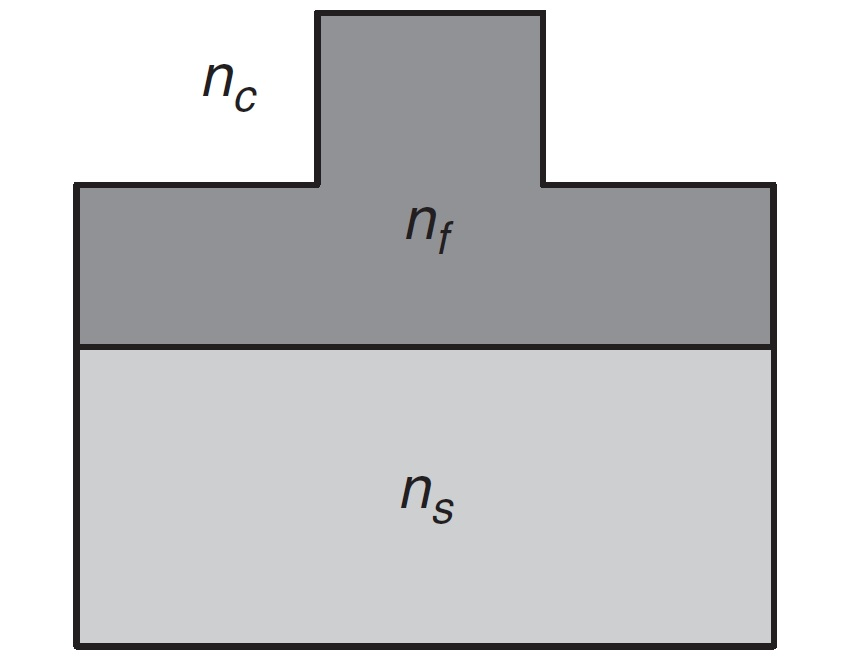
\includegraphics[width=\textwidth]{2-rib-wg}
		\caption{Rib waveguide}
		\label{fig:2_rib_wg}
	\end{subfigure}
	\hfill
	\begin{subfigure}[t]{0.3\textwidth}
		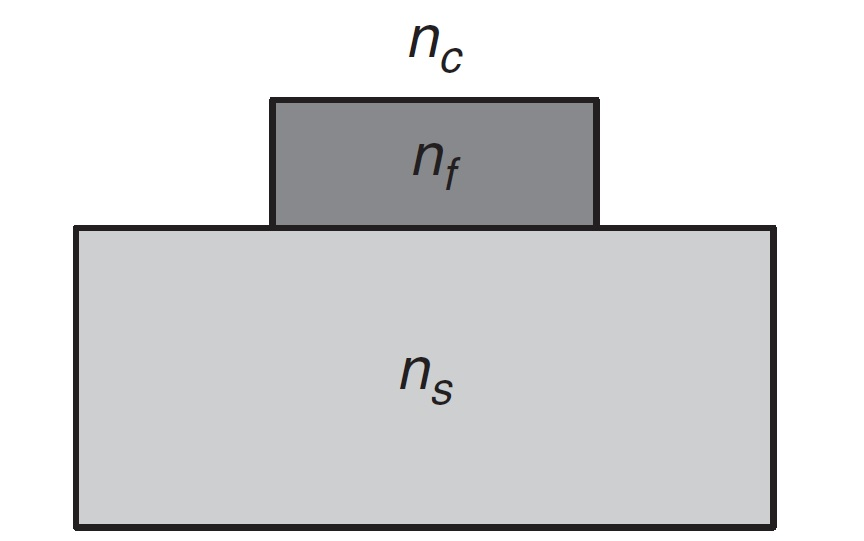
\includegraphics[width=\textwidth]{2-strip-wg}
		\caption{Strip waveguide}
		\label{fig:2_strip_wg}
	\end{subfigure}
	\hfill
	\begin{subfigure}[t]{0.3\textwidth}
		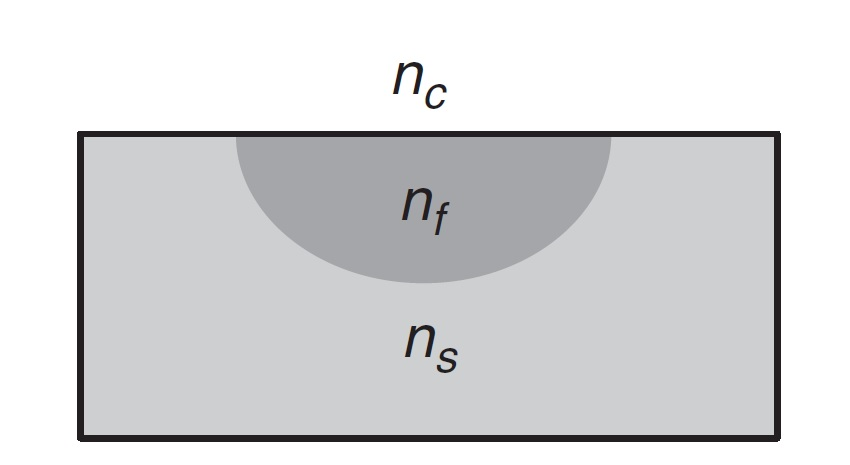
\includegraphics[width=\textwidth]{2-buried-wg}
		\caption{Buried waveguide}
		\label{fig:2_buried_wg}
	\end{subfigure}
	\caption{Different kinds of design for channel waveguides}
	\label{fig:2_waveguide_types}
\end{figure}
Different kinds of numerical methods like \gls{fem}, \gls{fit}, \gls{fdtd}, \gls{bpm} have been developed to decipher the nature of light propagation in channel waveguides.
	
	\begin{comment}
		\section{Snell's law and total internal reflection}
If light ray propagating in a medium with \gls{ri} $n_1$, impinges on the interface between two media, at an angle $\theta_1$, as shown in Figure \ref{fig:2_snells_law}, the ray is partially transmitted ($E_t$) and partially reflected ($E_r$). The relationship between the \gls{ri}s $n_1$ and $n_2$, and the angles of incidence ($\theta_1$) and refraction ($\theta_2$), is given by Snell's law:
\begin{equation}\label{eq:snells_law}
n_1 \sin \theta_1 = n_2 \sin \theta_2
\end{equation}
\begin{figure}[H]
	\centering
	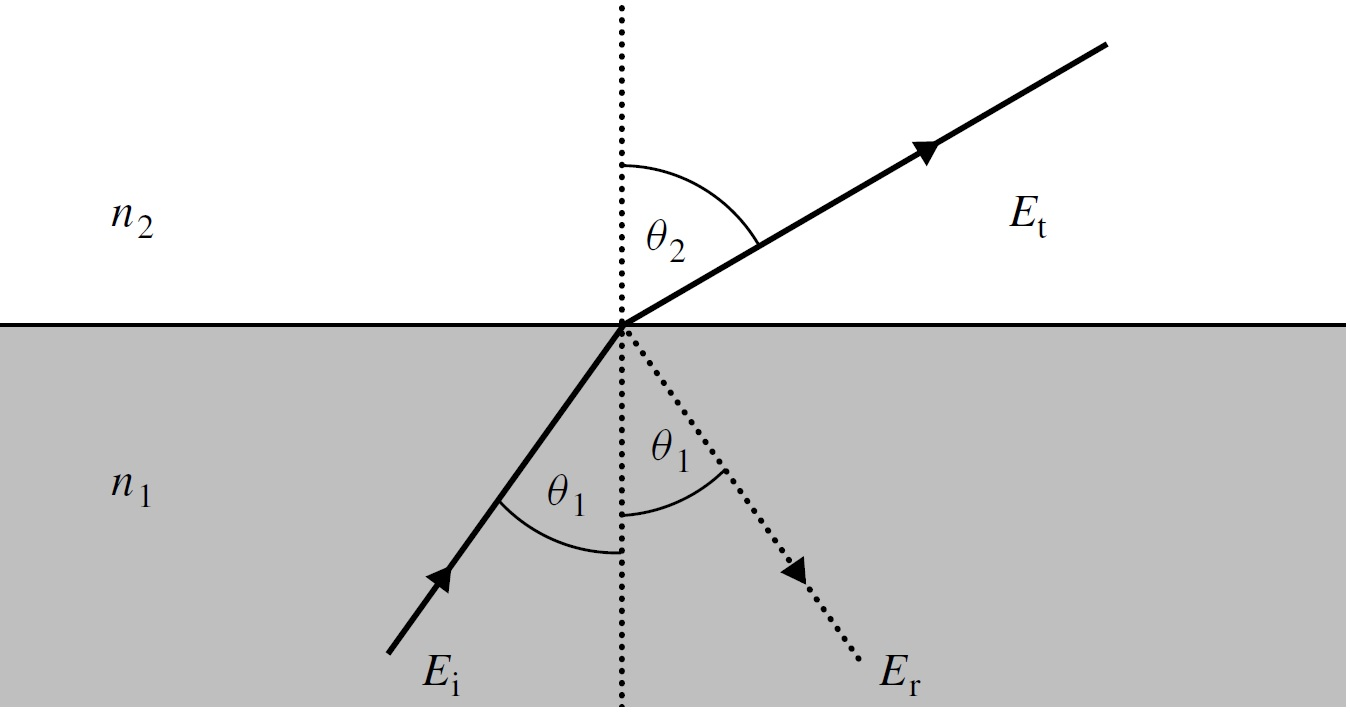
\includegraphics[width=0.75\textwidth]{2-snells-law}
	\caption{Light rays refracted and reflected at the interface of two media}
	\label{fig:2_snells_law}
\end{figure}
For some angle $\theta_1$, the corresponding angle $\theta_2$ will reach $90^{\circ}$, and hence Snell’s law simplifies to:
\begin{equation}\label{eq:critical angle}
\begin{aligned}
\begin{cases}
n_1 \sin \theta_c = n_2\\
\sin \theta_c = \dfrac{n_2}{n_1}
\end{cases}
\end{aligned}
\end{equation}
where, $\theta_c$ is defined as the critical angle. For angles of incidence greater than this critical angle, no light is transmitted and total internal reflection occurs. These properties are important to consider for finding the acceptance angle at which light can be inserted into a waveguide. The ray model helps in understanding of reflection and refraction of light at boundaries between the medium.
	\end{comment}
		
		\section{Eigenvalues and wave modes}
In general, the electric field and magnetic field in the wave equation in \ref{eq:wave_sol_electric} and \ref{eq:wave_sol_magnetic} can be written in its constituent parts in Cartesian coordinates as:
\begin{equation}\label{eq:em_field_cart_cord}
\begin{aligned}
\begin{cases}
\vec{E}=E_{x}i+E_{y}j+E_{z}k\\
\vec{H}=H_{x}i+H_{y}j+H_{z}k
\end{cases}
\end{aligned}
\end{equation}
The generalized vectorial component of the electric and magnetic field of equation \ref{eq:homogeneous_wave_sol_planar_wg} for a traveling wave in $Z$ direction can be combined into the Helmholtz equation as follows:
\begin{equation}\label{eq:helmholtz_eq_rib_wg}
	\begin{aligned}
		\nabla ^{2}\Psi \left( x,y,z\right) +k_{0}^{2}n^{2}\left(x,y\right) \Psi \left( x,y,z\right) = 0
	\end{aligned}
\end{equation}
where, $\Psi \left( x,y,z\right) = \psi \left( x,y\right)e^{-jkz} $ and then the equation \ref{eq:helmholtz_eq_rib_wg} can be rewritten as,
\begin{equation}\label{eq:helmholtz_eq_wg_general}
\begin{aligned}
\nabla_{xy} ^{2}\psi \left( x,y\right) +\left(k_{0}^{2}n^{2}\left(x,y\right) - k^2\right)\psi \left( x,y\right) = 0.
\end{aligned}
\end{equation}

\noindent The equation \ref{eq:helmholtz_eq_wg_general} can be solved for $\psi \left( x,y\right)$, using different numerical methods like \gls{fem}, \gls{fit}, \gls{bpm}, \gls{fdtd}. The numerical methods first decompose the waveguide into sufficient number small cells (more cells give more robust solution at the cost of increased computing turns) and then discretization of the refractive index profile is performed. Next the field equations are discretized by replacing the derivatives by their finite difference representations in those cells. In this way a set of linear equations are obtained which can be solved using standard algebraic methods. In general, \gls{fit} has a much lower memory footprint.\par

For given $\omega$, the resulting mode problem is an eigenproblem, solved for eigenvectors, i.e., mode profiles $\psi(x, y)$, and eigenvalues, from which the corresponding propagation constants $k$ of the modes are computed. The geometry of the waveguide is given by the transverse dependence of $\epsilon$, with effective \gls{ri} profile, and by appropriately chosen boundary conditions. Each allowed solution is referred to as the \textbf{mode of propagation}. For example, when light travels through a rectangular waveguide different modes can be visualized as follows in Fig. \ref{fig:2_rect_te_modes}.
\begin{figure}[H]
	\centering
	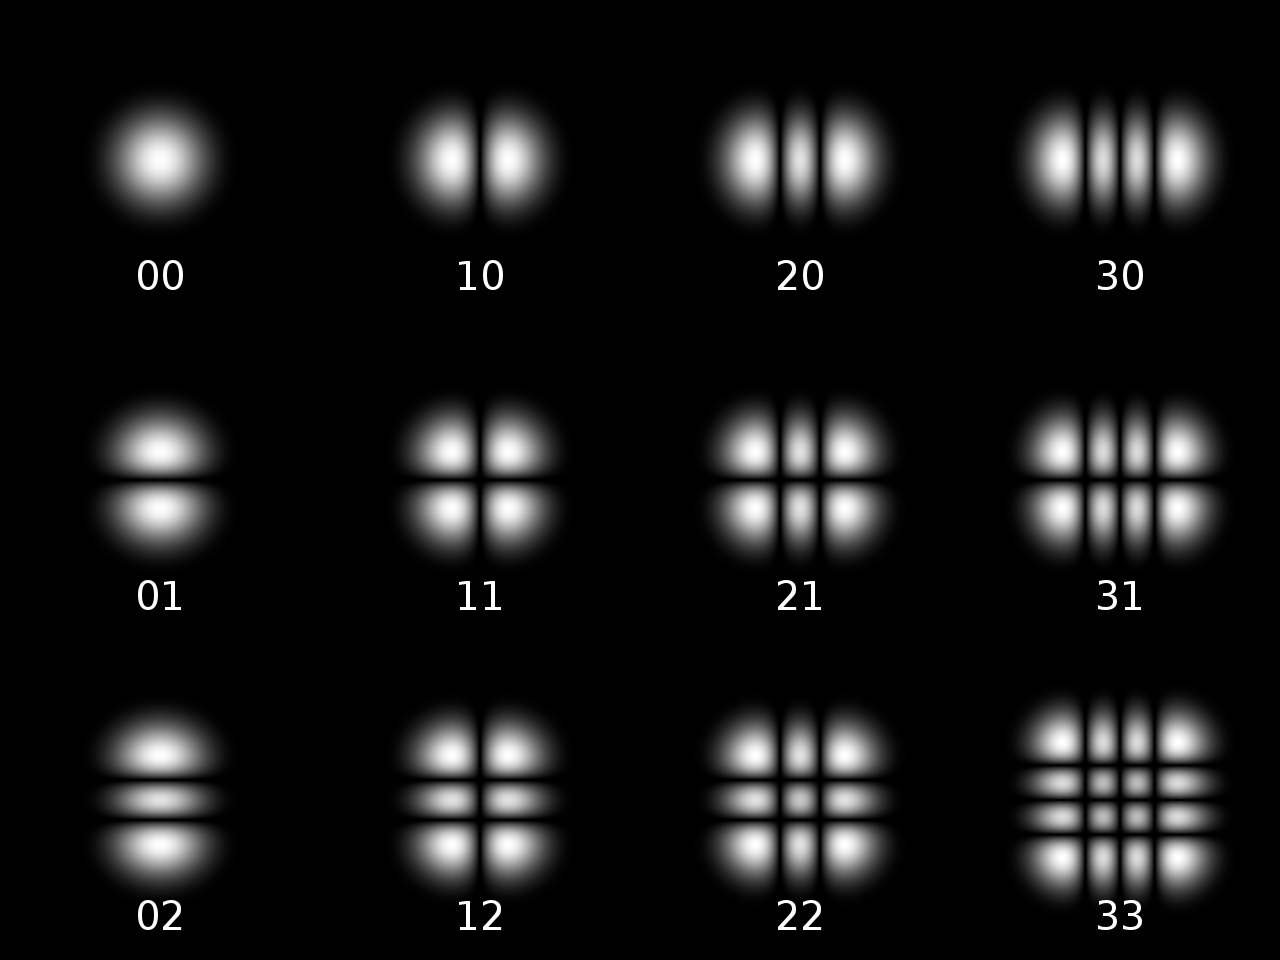
\includegraphics[width=0.75\textwidth]{2-rect-te-modes}
	\caption{TEM modes labelled with corresponding indices. The indices describe the shape of the modes as m+1 columns and n+1 rows. i.e. $\chem{TEM_{21}}$ mode shape has 3 columns and 2 rows.
	\label{fig:2_rect_te_modes}}
\end{figure}
		
		\section{Polarization}
Polarization is a wave mode solution which fits in the waveguide and is represented by the direction of the electric field associated with the propagating wave. In the example in Fig. \ref{fig:2_em_wave} the wave is linearly polarized since the electric field and magnetic field exist in one direction only. In a dielectric optical waveguide, light propagates in linearly polarized modes and the plane in which light is polarized is either vertical or horizontal to the direction of wave, as shown in Fig. \ref{fig:2_te_tm_mode} in single-mode.

	\begin{figure}[H]
		\centering
		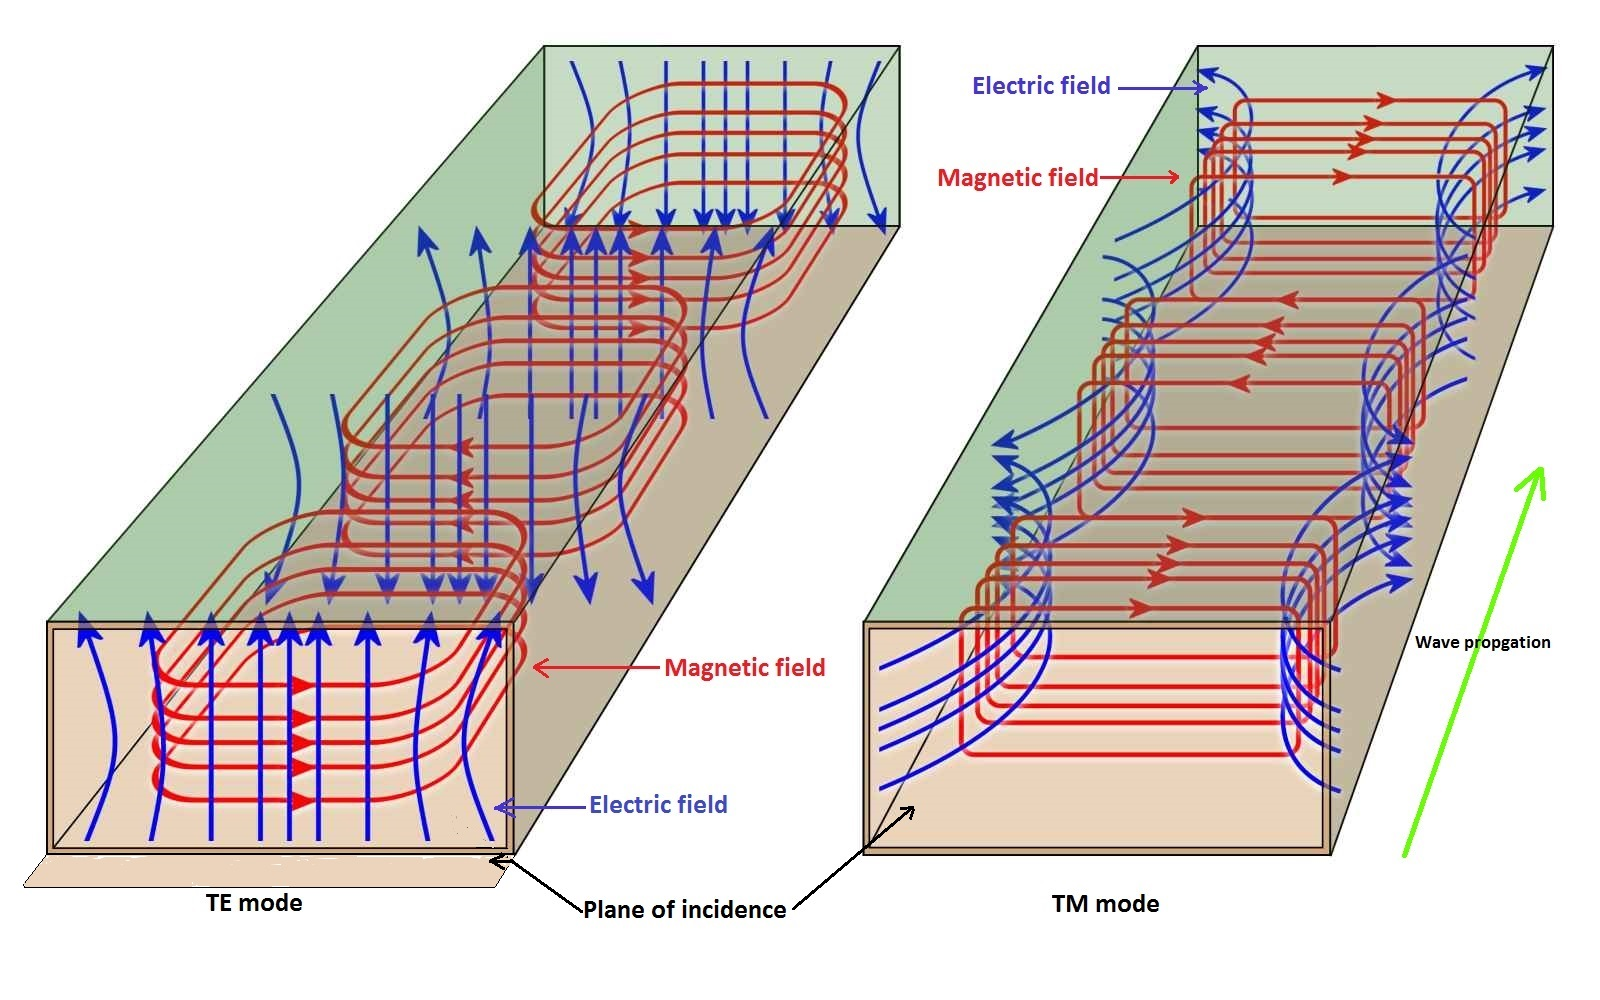
\includegraphics[width=\textwidth]{2-te-tm-mode}
		\caption{\gls{te} and \gls{tm} fundamental mode in a waveguide using CST simulation}
		\label{fig:2_te_tm_mode}
	\end{figure}	
			\subsection{TE mode}
\gls{te} mode is the fundamental mode in which there is no electric field in the direction of propagation of light wave. In Fig. \ref{fig:2_te_tm_mode} the electric field lines (blue) are perpendicular to the plane of incidence in \gls{te} mode. The plane of incidence is the plane in which optical waves strike the surface of the waveguide.						
			\subsection{TM mode}
\gls{tm} mode is the fundamental mode in which there is no magnetic field in the direction of propagation of light. In Fig. \ref{fig:2_te_tm_mode} it can be seen that magnetic field (red lines) are perpendicular to the plane of incidence in \gls{tm} mode.
 
			\subsection{Quasi-TE and Quasi-TM mode}				
Practically, waveguide cores have electric and magnetic fields that slice through air and the cladding substrate. Hence they do not support pure \gls{te} and \gls{tm} modes. However, since most the power is contained under the waveguide core and inside just the cladding, \gls{te} and \gls{tm} modes can be a good approximation. Generally, in these modes there is some field component in the direction of propagation as well. This is known as quasi-\gls{te} and quasi-\gls{tm} mode.
	
		\section{Jones calculus}
Polarized light can be represented using Jones calculus. Polarized light is represented using a \textit{Jones vector} and linear optical elements are represented by \textit{Jones matrices}.	When light crosses an optical element the resulting polarization of the emerging light is found by taking the product of the Jones matrix of the optical element and the Jones vector of the incident light. \textit{Jones calculus} is only applicable to light that is fully polarized \cite{burch_introduction_1975}.
		
			\subsection{Jones vector}
The Jones vector describes the \gls{sop} of light in free space or another homogeneous isotropic non-attenuating medium, where the light can be properly described as transverse waves \cite{burch_introduction_1975}. The Jones vector is a complex vector that is a mathematical representation of a real wave. A typical representation of the electric field for the optical wave described in \ref{eq:wave_sol_electric} can be as follows:
\begin{equation}\label{eq:jones_vector}
\vec{E} = \left( \begin{matrix} E_{x}\left( t\right) \\ E_{y}\left( t\right) \\ 0\end{matrix} \right) = \left( \begin{matrix} E_{x}e^{i\left( \omega t - kz+\phi _{x}\right)} \\ E_{y}e^{i\left( \omega t - kz+\phi _{y}\right) }\\ 0\end{matrix} \right) = \left( \begin{matrix} E_{x}e^{i\phi_x}\\ E_{y}e^{i\phi_y}\\ 0 \end{matrix} \right)e^{i\left( \omega t - kz\right)} 
\end{equation}
where $\phi_x$ and $\phi_y$ represent the phase of $E_x$ and $E_y$ fields. The Jones vector of the plane wave is described by:
\begin{equation}\label{eq:jones_vector_form}
\left( \begin{matrix} E_{x}e^{i\phi_x}\\ E_{y}e^{i\phi_y}\end{matrix} \right) 
\end{equation}
and the intensity of the optical wave, $I$ wave can be written as,
\begin{equation}\label{eq:jones_vector_intensity}
I = \left| E_x\right| ^{2}+\left| E_y\right| ^{2} 
\end{equation}
Generally, a wave of unit intensity is used for the consideration polarization. So Jones vector is noted using an unit vector as,
\begin{equation}\label{eq:jones_unit_vector_form}
	\vec{E}\overline {\vec{E}} = 1,
\end{equation}
where $\overline {E}$ is the complex conjugate of $E$. 
In general the Jones representation of a normalized elliptically polarized beam with azimuth $\theta$ and elliptical angle $\epsilon$ is given by,
\begin{equation}\label{eq:jones_vector_general_form}
e^{i\phi}\left(\begin{matrix} 
\cos\theta\cos\epsilon - j\sin\theta\sin\epsilon\\
\sin\theta\cos\epsilon - j\cos\theta\sin\epsilon 
\end{matrix} \right) 
\end{equation}
where $e^{i\phi}$ is an arbitrary phase vector and $\phi = \phi_x - \phi_y$. So, for example a linear polarization of \gls{te} mode can be represented as,
\begin{equation}\label{eq:jones_vector_linear_pol}
\left(\begin{matrix}  
1 \\
0
\end{matrix} \right) 
\end{equation}
since, $\theta=0$ and $\epsilon = 0$.
			
			\subsection{Jones matrix} \label{concept:jones_matrix}
Jones matrix is the formal representation of the various optical elements such as lenses, beam splitters, mirrors, phase retarders, polarizers at arbitrary angles that can modify polarization. They generally operate on Jones vectors and helps in comprehending situations which light encounters multiple polarization elements in sequence. In these situations the products of the Jones matrices can be used to represent the transfer matrix. This situation can be represented using,
\begin{equation}\label{eq:jones_matrix}
[E_{output}] = J_{system}[E_{input}] 
\end{equation}
where $E_{input}$ is the input field into the optical system and $E_{output}$ is the generated output field represented using Jones vector. The matrix $J_{system}$ is the Jones matrix of the optical system comprising of a series of polarization devices. If there are $N$ devices in the system then the final transfer matrix comes out as,
\begin{equation}\label{eq:jones_transfer_matrix}
J_{system} =J_{N}J_{N-1}\ldots \ldots J_{2}J_{1} 
\end{equation}   
where $J_{N}$ is the Jones matrix for $n^{th}$ polarizing optical element.

			\subsection{Jones matrix for polarizing optical systems}
Polarizer and wave plates are fundamental components which is required in an optical test-bench. These are discussed using Jones Calculus in the following sections.
		\subsubsection{Polarizer}
Polarizers have an index of refraction which depends on orientation electric field propagation. If any optical system has a transmission axis and an absorption axis for electric fields, then lights will be passed along the transmission axis and absorbed along the other axis. So, the Jones matrix of a polarizer making an angle $\theta$ with the X-axis will come out as,
\begin{equation}\label{eq:jones_matrix_polarizer}
\left(\begin{matrix} 
\cos ^{2}\theta & \sin \theta \cos \theta \\ 
\sin \theta \cos \theta & \sin ^{2}\theta
\end{matrix} \right) 
\end{equation} 
		\subsubsection{Wave plates}\label{concept:wave_plates}
Wave plates are phase retarders which are made of birefringent crystals. Wave plates can be conceptualized as two polarizers kept apart at certain distance $d$, such that their polarization axes are apart orthogonally ($90^{0}$). The phase difference as light passes through this setup of thickness $d$ is \cite{peatross_physics_2015},
\begin{equation}\label{eq:jones_matrix_wp1}
\left(k_{slow}-k_{fast}\right)d = \dfrac {2\pi d} {\lambda_{vac} }\left( n_{slow}-n_{fast}\right) 
\end{equation}
In, general the Jones matrix for a wave plate is given by \cite{peatross_physics_2015},
\begin{equation}\label{eq:jones_matrix_wp2}
\left( \begin{matrix} 
\cos ^{2}\theta +\xi \sin ^{2}\theta & \sin \theta \cos \theta -\xi \sin \theta \cos \theta\\ 
\sin \theta \cos \theta -\xi \sin \theta \cos \theta & \sin ^{2}\theta +\xi \cos ^{2}\theta
\end{matrix} \right) 
\end{equation}
where $\xi$ is calculated based on the type of wave plate. The following equations addresses some specific scenarios:
\begin{equation}\label{eq:jones_matrix_wp3}
\begin{aligned}
\begin{cases} 
\xi = e^{i\pi/2}, \,\quad \text{where,} \left(k_{slow}-k_{fast}\right)d = \pi/2 + 2\pi m, \text{for quarter-wave plate}\\ 
\xi = e^{i\pi},  \;\;\;\quad \text{where,} \left(k_{slow}-k_{fast}\right)d = \pi + 2\pi m, \text{for half-wave plate}
\end{cases}
\end{aligned}
\end{equation}
and $m \in \mathbb{Z}$. $\xi$ is the phase delay of the wave plates. Similar concept is used in the construction of \gls{pr} waveguides which will be discussed in later sections shortly.
 		
		\section{Poincaré sphere and state of polarization} \label{concept:poincare_sphare}
To view a complete representation of all the polarization ellipses generated using Jones vectors, a spherical structure with unit radius is used, which is known as Poincaré sphere. If the orientation in space of of the ellipse of polarization is determined by the azimuth, $\theta$ and ellipticity, $\epsilon$ then that point can be completely characterized by its longitude $2\theta$ and latitude $2\epsilon$. The north and south poles represent the right-handed and left-handed circular polarization respectively. In general the diametrically opposite points represent pairs of orthogonal polarization. The \gls{sop} and its corresponding location in the Poincaré sphere is visualized in the Fig. \ref{fig:2_poincare}. To go from one \gls{sop} to another the polarized light can be passed through various optical components which can be computed using the Jones matrix and the corresponding \gls{sop} can be represented on the Poincaré sphere. 
     
\begin{figure}[H]
	\centering
	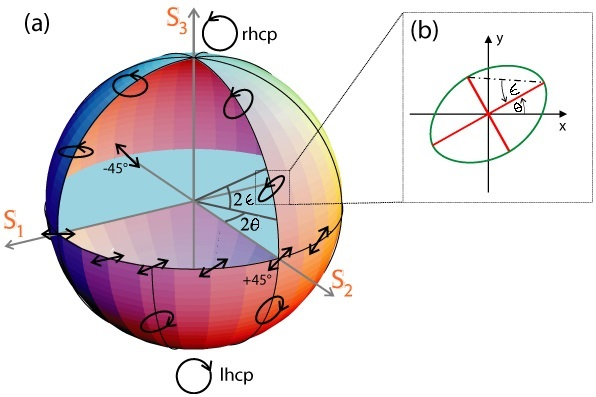
\includegraphics[width=0.75\textwidth]{2-poincare}
	\caption{(a) Representation of the Poincaré sphere (b) Representation of the ellipse parameters \cite{flossmann_stokes_2006}}
	\label{fig:2_poincare}
\end{figure}
\noindent For complete polarized light, the point on the Poincaré sphere must be fixed on time which requires,
\begin{equation}\label{eq:polarization_condition_1}
\dfrac {E_{x}\left( t\right) } {E_{y}\left( t\right) }=constant
\end{equation}
and,
\begin{equation}\label{eq:polarization_condition_2}
\phi = \phi_{x}(t) - \phi_{y}(t)=constant
\end{equation}
  
		\section{Stoke's parameter} 		
Quasi-monochromatic waves are mathematically treated using Stokes parameters ($S_0,S_1,S_2,S_3$), which constitute a vector generally known as Stokes vectors. Stokes vectors are used to keep track of the partial polarization (and attenuation) of a light beam in terms of total intensity (I), degree of polarization (p) and ellipse parameters, as the light progresses through an optical system. A Stokes vector can generally be represented as,
\begin{equation}\label{eq:stokes_vector}
\overrightarrow {S} = \left(\begin{matrix}  
	S_0 \\
	S_1 \\
	S_2 \\
	S_3
\end{matrix} \right) 
\end{equation}
where,
\begin{equation}\label{eq:stokes_parameters}
\begin{aligned}
\begin{cases}
S_{0}=I\\ 
S_{1}=I_{p}\cos 2\theta \cos 2\epsilon \\
S_{2}=I_{p}\sin 2\theta \cos 2\epsilon \\
S_{3}=I_{p}\sin 2\epsilon
\end{cases}
\end{aligned}
\end{equation}
Here, $I_p, 2\theta, 2\epsilon$ are the spherical coordinates of the 3-D vector of Cartesian coordinates $(S_1,S_2,S_3)$. So, given the Stokes parameters, the spherical coordinates $(p,2\theta,2\epsilon)$ can be obtained and represented by a point inside the Poincaré sphere using the following:
\begin{equation}\label{eq:stokes_spherical_coordinates}
\begin{aligned}
\begin{cases}
I = S_{0}\\ 
p = \dfrac {\sqrt {S_{1}^{2}+S_{2}^{2}+S_{3}^{2}}} {S_{0}} \\
2\theta = \tan^{-1}\dfrac {S_{2}} {S_{1}} \\
2\epsilon = \tan ^{-1}\dfrac {S_{3}} {\sqrt {S_{1}^{2}+S_{2}^{2}}}
\end{cases}
\end{aligned}
\end{equation}
The prescribed notations are portrayed on the Poincaré sphere in the following Fig. \ref{fig:2_stoke_param_poincare_sphere}.    
\begin{figure}[H]
	\centering
	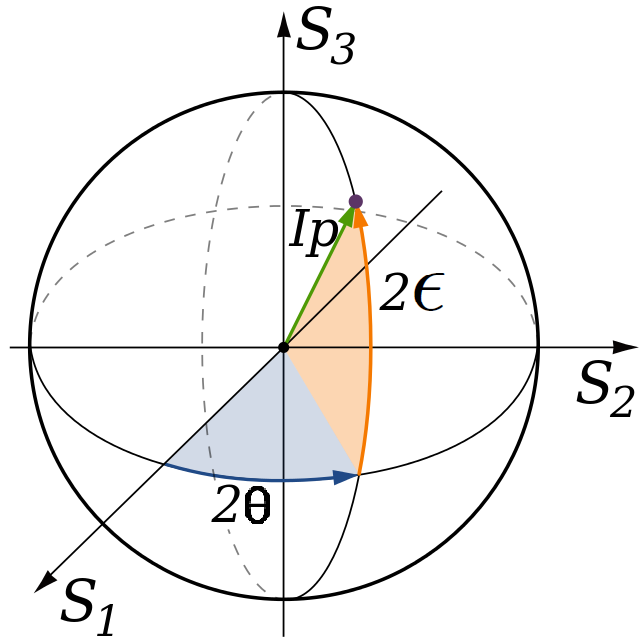
\includegraphics[width=0.50\textwidth]{2-stoke-param-poincare-sphere}
	\caption{Poincaré sphere, on or beneath which the three Stokes parameters [S1, S2, S3] are plotted in Cartesian coordinates \cite{stoke_poincare_parameter}}
	\label{fig:2_stoke_param_poincare_sphere}
\end{figure}

	\section{Coupled mode theory}\label{concept:mode_coupling}
In a waveguide, an ideal mode is an eigenvector of a propagation constant. Mode coupling enables transfer of energy from one ideal mode to another, during propagation. Mode coupling can be induced by introducing another independent waveguide structure in close proximity (coupled waveguides in close proximity are modeled as a single structure, forming supermodes). The pairwise coupling strength between two modes depends on a dimensionless ratio between the coupling coefficient (per unit length) and the difference between the two modal propagation constants. Hence, a given perturbation may strongly couple modes having nearly equal propagation constants, but weakly couple modes having highly unequal propagation constants. \gls{pmd} and \gls{pdl} have long been described by field coupling models, in which phase dependent coupling of modal fields is described by complex coefficients. Field coupling models describe not only a redistribution of energy among modes, but also how eigenvectors and their eigenvalues depend on the mode coupling coefficients \cite{kahn_mode_2012}.

\paragraph*{Perturbation Analysis:}
Supermodes can be represented as weighted sum of individual guided modes. If two modes are represented by $\psi_1(x,y)$ and $\psi_2(x,y)$ in the different waveguides along with the coupling between two modes as $X_i(z)$, then the supermode can be written using Helmholtz identity as, 
\begin{equation}\label{eq:supermodes}
	\Psi(x,y,z) = X_1(z)\psi_1(x,y) + X_2(z)\psi_2(x,y)
\end{equation} 	
The uncoupled modes, $\psi_1$ and $\psi_2$ satisfy the following propagation equations with propagation constants $k_1$ and $k_2$,
\begin{equation}\label{eq:uncoupled_mode}
\begin{aligned}
\begin{cases}
\dfrac {dX_{1}} {dz}=-jk_{1}X_{1} \\[10pt]
\dfrac {dX_{2}} {dz}=-jk_{2}X_{2}
\end{cases}
\end{aligned}
\end{equation}
A known solution for \ref{eq:uncoupled_mode} is:
\begin{equation}\label{eq:uncoupled_mode_sol}
\begin{aligned}
\begin{cases}
X_{1} (z) = e ^ {-jk_{1}z} \\
X_{2} (z) = e ^ {-jk_{2}z}
\end{cases}
\end{aligned}
\end{equation}
Coupled mode theory postulates that to describe a perturbed system the linear coupling terms need to be added as,
\begin{equation}\label{eq:coupled_mode_sol}
\begin{aligned}
\begin{cases}
\dfrac {dX_{1}} {dz} = -jk_{1}X_{1}(z) - j(\kappa_{11}X_1+\kappa_{12}X_2) \\[10pt]
\dfrac {dX_{2}} {dz} = -jk_{2}X_{2}(z) - j(\kappa_{21}X_1+\kappa_{22}X_2)
\end{cases}
\end{aligned}
\end{equation}
where, $\kappa_{ij}$, $\forall \left( i,j\right) \in \left[ 1,2\right] $  are the linear coefficients which can be understood using the scattering matrix as,
\begin{equation}\label{eq:scattering_matix_coupler}
\left(\begin{matrix} 
\kappa_{11} & \kappa_{12} \\ 
\kappa_{21} & \kappa_{22}
\end{matrix} \right) 
\end{equation} 
where,
\begin{equation}\label{eq:coupled_mode_coupling_coeff}
\begin{aligned}
\begin{cases}
\kappa_{11} = \dfrac{1}{2}k_0^2\int\int(n_{12}^2-n_{1}^2)\psi_1^2dxdy \\[10pt]
\kappa_{12} = \dfrac{1}{2}k_0^2\int\int(n_{12}^2-n_{1}^2)\psi_1\psi_2 dxdy \\[10pt]
\kappa_{21} = \dfrac{1}{2}k_0^2\int\int(n_{12}^2-n_{2}^2)\psi_1\psi_2 dxdy \\[10pt]
\kappa_{22} = \dfrac{1}{2}k_0^2\int\int(n_{12}^2-n_{2}^2)\psi_2^2 dxdy
\end{cases}
\end{aligned}
\end{equation}	
Here, $\kappa_{11}$ and $\kappa_{22}$ are the reflection coefficients and $\kappa_{12}$ and $\kappa_{21}$ are the coupling coefficients. Normally, it is assumed that the modes are normalized, and propagate in a lossless system with symmetric coupling coefficients. Hence,
\begin{equation}\label{eq:symmetric_coupling_coeff}
\kappa_{12} = \kappa_{21} 
\end{equation}
Coupling coefficients and phase mismatch are important factors for power exchange between different modes. In \ref{fig:2_mc_theory_1} both the waveguides are excited where as in \ref{fig:2_mc_theory_2} only waveguide $B$ is excited.
\begin{figure}[H]
	\begin{subfigure}[t]{0.45\textwidth}
		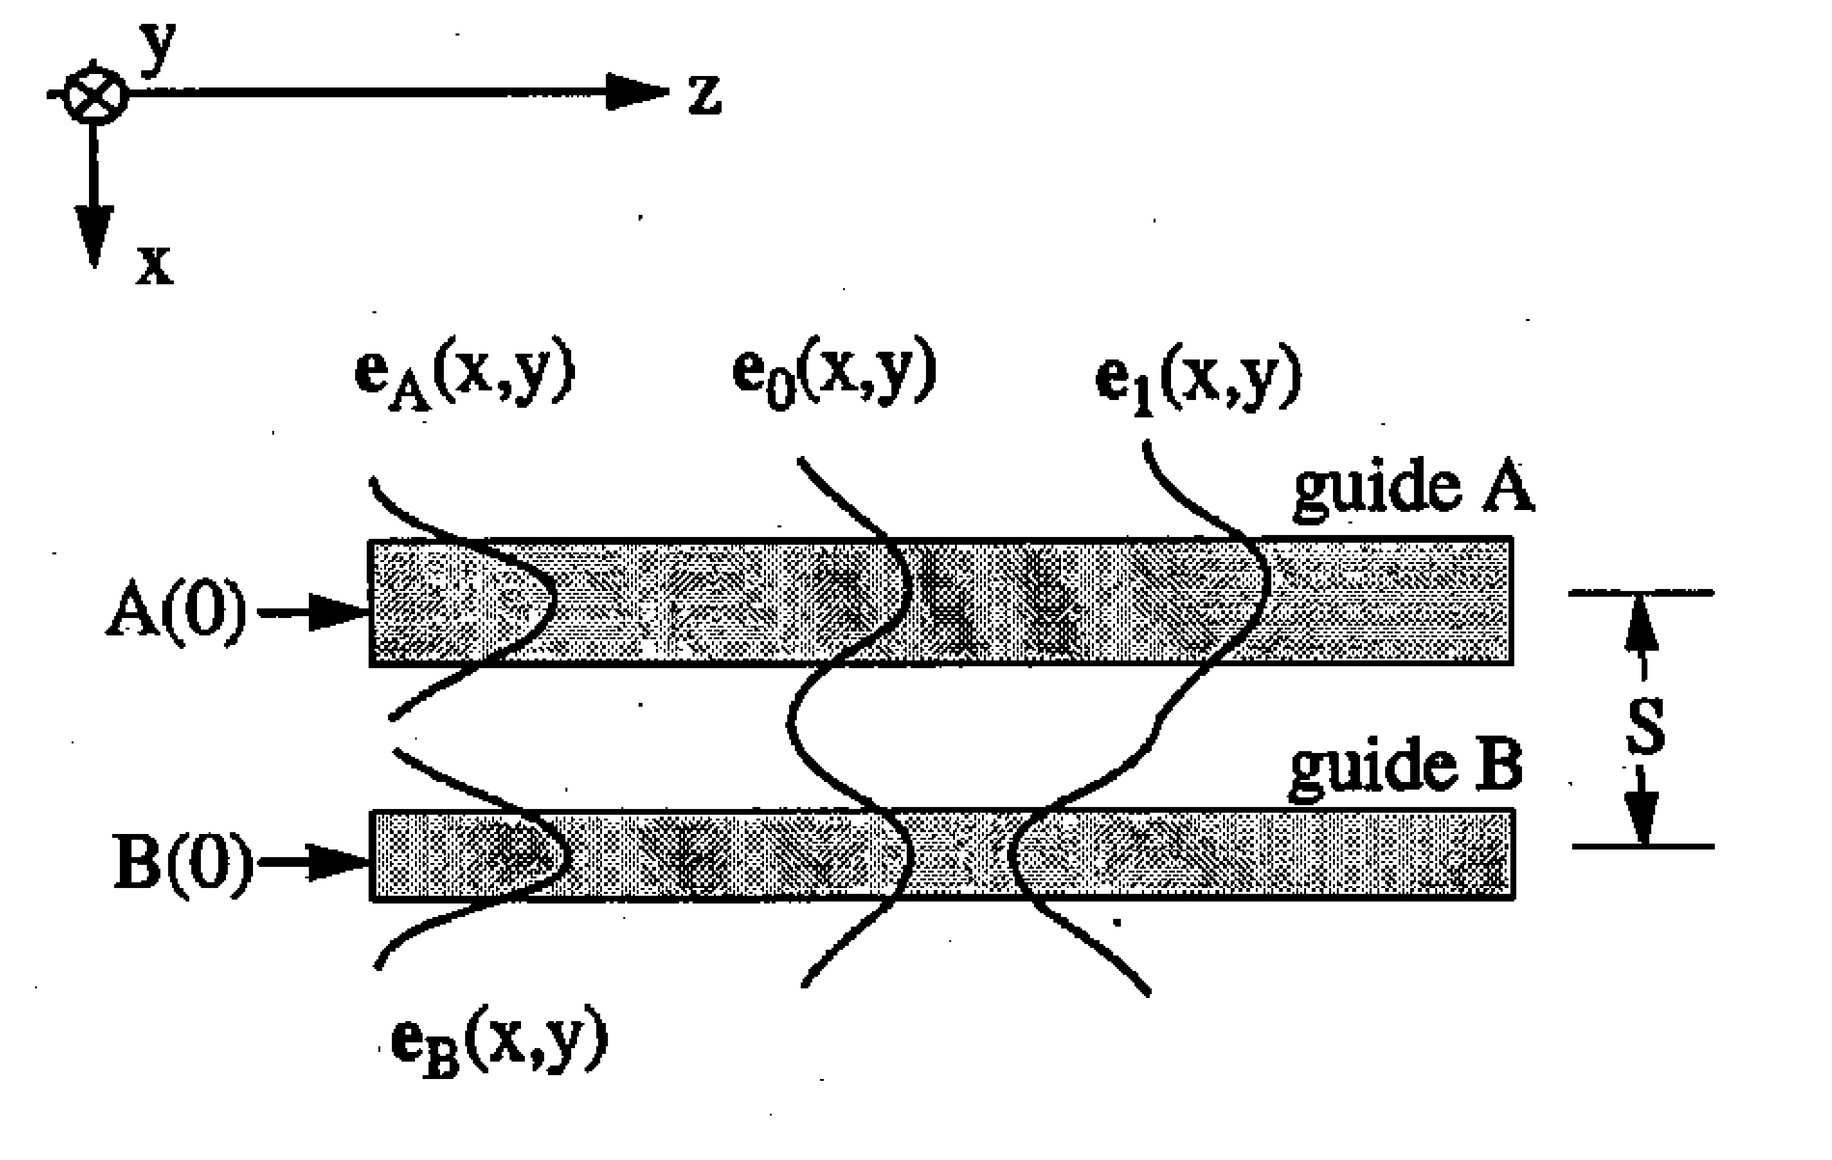
\includegraphics[width=\textwidth]{2-mc-theory-1}
		\caption{Individual and normal modes in two different waveguides}
		\label{fig:2_mc_theory_1}
	\end{subfigure}
	\hfill
	\begin{subfigure}[t]{0.45\textwidth}
		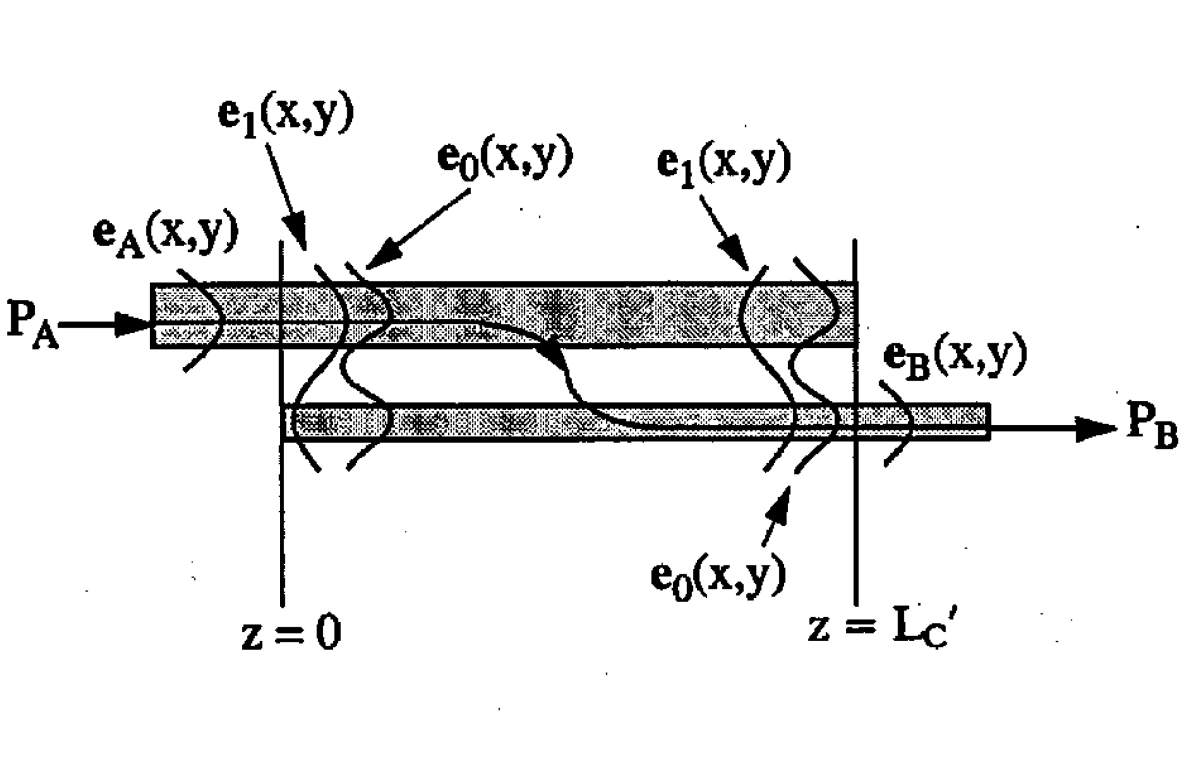
\includegraphics[width=\textwidth]{2-mc-theory-2}
		\caption{Power transfer from arm $A$ to arm $B$ by normal-mode coupling}
		\label{fig:2_mc_theory_2}
	\end{subfigure}
	\caption{Description of the directional coupler under coupled-mode and normal-mode}
\end{figure}

\noindent In \ref{fig:2_mc_theory_2} for no phase mismatch complete power exchange occurs. This is why phase matching is an important criteria for mode coupling. The coupling length is, $L_c = \pi / 2\kappa$. 

\par 
Coupling mode theory has been successfully applied to the modeling and analysis of various guided-wave optoelectronic devices, such as optical directional couplers made of thin film and channel waveguides, multiple waveguide lenses, phase-locked laser arrays, distributed feedback lasers and distributed Bragg reflectors, grating waveguides and couplers, nonparallel and tapered waveguide structures, Y-branch waveguides, \gls{te}/\gls{tm} polarization converters, mode conversion and radiation loss in slab waveguides, residual coupling among scalar modes. It has also been used to study the wave coupling phenomena in nonlinear media such as harmonic generation in bulk and guided-wave devices, and nonlinear coherent couplers \cite{haus_coupled_1991}.

\section{Figures of merit}
The \gls{fom} represents the benchmarks present for comparing different optical waveguide components.			
\subsection{Confinement factor}
The confinement factor is a measure of the proportion of the electric field power in a given mode that lies within the core.  
\begin{equation}\label{eq:per}
\text{ Confinement factor } = \dfrac {\int _{-w / 2}^{w/2}E_{x}^{2}\left( y\right) dy} {\int _{-\infty }^{\infty }E_{x}^{2}\left( y\right) dy},
\end{equation}
where, $w$ is the width of the waveguide core. Confinement factor is an important measure which is function of various factors like polarization, \gls{ri} difference between the core and cladding, mode number etc.	

\subsection{Polarization extinction ratio}
The \gls{per} is the ratio of optical powers of \gls{te} and \gls{tm} polarizations. The \gls{per} is used to characterize the degree of polarization in a polarization maintaining device or fiber. 	
\begin{equation}\label{eq:wave_sop}
\begin{aligned}
\begin{cases}
PER_{TE-TM} = 10\log_{10} \dfrac {P_{TM}} {P_{TE}}\\
PER_{TM-TE} = 10\log_{10} \dfrac {P_{TE}} {P_{TM}}
\end{cases}
\end{aligned}
\end{equation}

\subsection{Insertion loss}
Insertion loss is the loss of signal power resulting from the insertion of a device in a transmission line or optical fiber and is usually expressed in decibels (dB). If the power transmitted to the load before insertion is $P_{in}$ and the power received by the load after insertion is $P_{out}$, then the \gls{il} in dB is given by,
\begin{equation}\label{eq:insertion_loss}
\gls{il} = 10\log _{10} \dfrac {P_{in}} {P_{out}}
\end{equation}
\end{document}
